% Options for packages loaded elsewhere
\PassOptionsToPackage{unicode}{hyperref}
\PassOptionsToPackage{hyphens}{url}
%
\documentclass[
  a4paper,
]{book}

\usepackage{amsmath,amssymb}
\usepackage{iftex}
\ifPDFTeX
  \usepackage[T1]{fontenc}
  \usepackage[utf8]{inputenc}
  \usepackage{textcomp} % provide euro and other symbols
\else % if luatex or xetex
  \usepackage{unicode-math}
  \defaultfontfeatures{Scale=MatchLowercase}
  \defaultfontfeatures[\rmfamily]{Ligatures=TeX,Scale=1}
\fi
\usepackage{lmodern}
\ifPDFTeX\else  
    % xetex/luatex font selection
\fi
% Use upquote if available, for straight quotes in verbatim environments
\IfFileExists{upquote.sty}{\usepackage{upquote}}{}
\IfFileExists{microtype.sty}{% use microtype if available
  \usepackage[]{microtype}
  \UseMicrotypeSet[protrusion]{basicmath} % disable protrusion for tt fonts
}{}
\makeatletter
\@ifundefined{KOMAClassName}{% if non-KOMA class
  \IfFileExists{parskip.sty}{%
    \usepackage{parskip}
  }{% else
    \setlength{\parindent}{0pt}
    \setlength{\parskip}{6pt plus 2pt minus 1pt}}
}{% if KOMA class
  \KOMAoptions{parskip=half}}
\makeatother
\usepackage{xcolor}
\usepackage[top=35mm,right=25mm,bottom=35mm,left=25mm,heightrounded]{geometry}
\setlength{\emergencystretch}{3em} % prevent overfull lines
\setcounter{secnumdepth}{-\maxdimen} % remove section numbering
% Make \paragraph and \subparagraph free-standing
\makeatletter
\ifx\paragraph\undefined\else
  \let\oldparagraph\paragraph
  \renewcommand{\paragraph}{
    \@ifstar
      \xxxParagraphStar
      \xxxParagraphNoStar
  }
  \newcommand{\xxxParagraphStar}[1]{\oldparagraph*{#1}\mbox{}}
  \newcommand{\xxxParagraphNoStar}[1]{\oldparagraph{#1}\mbox{}}
\fi
\ifx\subparagraph\undefined\else
  \let\oldsubparagraph\subparagraph
  \renewcommand{\subparagraph}{
    \@ifstar
      \xxxSubParagraphStar
      \xxxSubParagraphNoStar
  }
  \newcommand{\xxxSubParagraphStar}[1]{\oldsubparagraph*{#1}\mbox{}}
  \newcommand{\xxxSubParagraphNoStar}[1]{\oldsubparagraph{#1}\mbox{}}
\fi
\makeatother
\pagestyle{plain}


\providecommand{\tightlist}{%
  \setlength{\itemsep}{0pt}\setlength{\parskip}{0pt}}\usepackage{longtable,booktabs,array}
\usepackage{calc} % for calculating minipage widths
% Correct order of tables after \paragraph or \subparagraph
\usepackage{etoolbox}
\makeatletter
\patchcmd\longtable{\par}{\if@noskipsec\mbox{}\fi\par}{}{}
\makeatother
% Allow footnotes in longtable head/foot
\IfFileExists{footnotehyper.sty}{\usepackage{footnotehyper}}{\usepackage{footnote}}
\makesavenoteenv{longtable}
\usepackage{graphicx}
\makeatletter
\newsavebox\pandoc@box
\newcommand*\pandocbounded[1]{% scales image to fit in text height/width
  \sbox\pandoc@box{#1}%
  \Gscale@div\@tempa{\textheight}{\dimexpr\ht\pandoc@box+\dp\pandoc@box\relax}%
  \Gscale@div\@tempb{\linewidth}{\wd\pandoc@box}%
  \ifdim\@tempb\p@<\@tempa\p@\let\@tempa\@tempb\fi% select the smaller of both
  \ifdim\@tempa\p@<\p@\scalebox{\@tempa}{\usebox\pandoc@box}%
  \else\usebox{\pandoc@box}%
  \fi%
}
% Set default figure placement to htbp
\def\fps@figure{htbp}
\makeatother

\flushbottom
\makeatletter
\@ifpackageloaded{bookmark}{}{\usepackage{bookmark}}
\makeatother
\makeatletter
\@ifpackageloaded{caption}{}{\usepackage{caption}}
\AtBeginDocument{%
\ifdefined\contentsname
  \renewcommand*\contentsname{Inhaltsverzeichnis}
\else
  \newcommand\contentsname{Inhaltsverzeichnis}
\fi
\ifdefined\listfigurename
  \renewcommand*\listfigurename{Abbildungsverzeichnis}
\else
  \newcommand\listfigurename{Abbildungsverzeichnis}
\fi
\ifdefined\listtablename
  \renewcommand*\listtablename{Tabellenverzeichnis}
\else
  \newcommand\listtablename{Tabellenverzeichnis}
\fi
\ifdefined\figurename
  \renewcommand*\figurename{Abbildung}
\else
  \newcommand\figurename{Abbildung}
\fi
\ifdefined\tablename
  \renewcommand*\tablename{Tabelle}
\else
  \newcommand\tablename{Tabelle}
\fi
}
\@ifpackageloaded{float}{}{\usepackage{float}}
\floatstyle{ruled}
\@ifundefined{c@chapter}{\newfloat{codelisting}{h}{lop}}{\newfloat{codelisting}{h}{lop}[chapter]}
\floatname{codelisting}{Listing}
\newcommand*\listoflistings{\listof{codelisting}{Listingverzeichnis}}
\makeatother
\makeatletter
\makeatother
\makeatletter
\@ifpackageloaded{caption}{}{\usepackage{caption}}
\@ifpackageloaded{subcaption}{}{\usepackage{subcaption}}
\makeatother
\makeatletter
\@ifpackageloaded{sidenotes}{}{\usepackage{sidenotes}}
\@ifpackageloaded{marginnote}{}{\usepackage{marginnote}}
\makeatother

\ifLuaTeX
\usepackage[bidi=basic]{babel}
\else
\usepackage[bidi=default]{babel}
\fi
\babelprovide[main,import]{ngerman}
% get rid of language-specific shorthands (see #6817):
\let\LanguageShortHands\languageshorthands
\def\languageshorthands#1{}
\ifLuaTeX
  \usepackage[german]{selnolig} % disable illegal ligatures
\fi
\usepackage{bookmark}

\IfFileExists{xurl.sty}{\usepackage{xurl}}{} % add URL line breaks if available
\urlstyle{same} % disable monospaced font for URLs
\hypersetup{
  pdftitle={Demo V2 Layouts},
  pdfauthor={ASKCR},
  pdflang={de},
  hidelinks,
  pdfcreator={LaTeX via pandoc}}


\title{Demo V2 Layouts}
\author{ASKCR}
\date{2025-02-07}

\begin{document}
\frontmatter
\maketitle

\renewcommand*\contentsname{Inhaltsverzeichnis}
{
\setcounter{tocdepth}{2}
\tableofcontents
}

\mainmatter
\bookmarksetup{startatroot}

\chapter{Katalog zur Ausstellung: Der Große Saal
(Rittersaal)}\label{katalog-zur-ausstellung-der-grouxdfe-saal-rittersaal}

Ein Katalog mit Kunstwerken aus der CbDD-Sammlung. Textteil:
\href{https://www.deckenmalerei.eu/42d06165-58e7-4653-bfe4-3d5f7091fc33\#6e73f774-4b7f-4e37-937b-e11cc35c5bc8}{6e73f774-4b7f-4e37-937b-e11cc35c5bc8}

Großer Saal (Rittersaal) {[}Raum{]}

This work is licensed under a Creative Commons
Attribution-NonCommercial-NoDerivs 4.0 International License.

\bookmarksetup{startatroot}

\chapter{Gallery Map}\label{gallery-map}

\begin{verbatim}
<folium.folium.Map at 0x1a52c44a410>
\end{verbatim}

\bookmarksetup{startatroot}

\chapter{Gallery Full Image}\label{gallery-full-image}

\phantomsection\label{infogrid}
\phantomsection\label{paintingName}

\phantomsection\label{paintingYear}

\phantomsection\label{paintingSize}{} {Wikidata}

\bookmarksetup{startatroot}

\chapter{Gallery Masonry}\label{gallery-masonry}

\phantomsection\label{http:ux2fux2fwww.wikidata.orgux2fentityux2fQ105576317}
Wrapped in Loveby: Israel Tsvaygenbaum2014

\begin{figure}[H]

{\centering \includegraphics[width=\linewidth,height=10cm,keepaspectratio]{index_files/mediabag/Israel-Tsvaygenbaum-.jpg}

}

\caption{image}

\end{figure}%

\phantomsection\label{http:ux2fux2fwww.wikidata.orgux2fentityux2fQ55852280}
Passarola de Bartolomeu de Gusmãoby: José Wasth Rodrigues2000

\begin{figure}[H]

{\centering \includegraphics[width=\linewidth,height=10cm,keepaspectratio]{index_files/mediabag/José-Wasth-Rodrigue.jpg}

}

\caption{image}

\end{figure}%

\phantomsection\label{http:ux2fux2fwww.wikidata.orgux2fentityux2fQ55852494}
Passarola de Bartolomeu de Gusmãoby: José Wasth Rodrigues2000

\begin{figure}[H]

{\centering \includegraphics[width=\linewidth,height=10cm,keepaspectratio]{index_files/mediabag/José-Wasth-Rodrigue1.jpg}

}

\caption{image}

\end{figure}%

\phantomsection\label{http:ux2fux2fwww.wikidata.orgux2fentityux2fQ56807932}
Okutatami Lakeby: Li Mei-shu1980

\begin{figure}[H]

{\centering \includegraphics[width=\linewidth,height=10cm,keepaspectratio]{index_files/mediabag/Okutatami-Lake.jpg}

}

\caption{image}

\end{figure}%

\phantomsection\label{http:ux2fux2fwww.wikidata.orgux2fentityux2fQ19917454}
Seneca Lakeby: Arthur Dove1935

\begin{figure}[H]

{\centering \includegraphics[width=\linewidth,height=10cm,keepaspectratio]{index_files/mediabag/Seneca-Lake-MET-DP23.jpg}

}

\caption{image}

\end{figure}%

\phantomsection\label{http:ux2fux2fwww.wikidata.orgux2fentityux2fQ50776315}
Q50776315by: Villem Ormisson1934

\begin{figure}[H]

{\centering \includegraphics[width=\linewidth,height=10cm,keepaspectratio]{index_files/mediabag/Varemed,-Villem-Ormi.jpg}

}

\caption{image}

\end{figure}%

\phantomsection\label{http:ux2fux2fwww.wikidata.orgux2fentityux2fQ20491060}
Buffalo Sceneby: Emil W. Lenders1922

\begin{figure}[H]

{\centering \includegraphics[width=\linewidth,height=10cm,keepaspectratio]{index_files/mediabag/Emil-W.-Lenders---Bu.jpg}

}

\caption{image}

\end{figure}%

\phantomsection\label{http:ux2fux2fwww.wikidata.orgux2fentityux2fQ50790393}
Q50790393by: Konrad Mägi1922

\begin{figure}[H]

{\centering \includegraphics[width=\linewidth,height=10cm,keepaspectratio]{index_files/mediabag/Konrad-Mägi-TKM-007.jpg}

}

\caption{image}

\end{figure}%

\phantomsection\label{http:ux2fux2fwww.wikidata.orgux2fentityux2fQ20191641}
A Stormby: Georgia O'Keeffe1922

\begin{figure}[H]

{\centering \includegraphics[width=\linewidth,height=10cm,keepaspectratio]{index_files/mediabag/A-Storm-DT1394.jpg}

}

\caption{image}

\end{figure}%

\phantomsection\label{http:ux2fux2fwww.wikidata.orgux2fentityux2fQ64686030}
Lake and mountainsby: John Kelt Edwards1920

\begin{figure}[H]

{\centering \includegraphics[width=\linewidth,height=10cm,keepaspectratio]{index_files/mediabag/Lake-and-mountains.jpg}

}

\caption{image}

\end{figure}%

\phantomsection\label{http:ux2fux2fwww.wikidata.orgux2fentityux2fQ20795141}
Small Lakeby: Magnus Enckell1919

\begin{figure}[H]

{\centering \includegraphics[width=\linewidth,height=10cm,keepaspectratio]{index_files/mediabag/Magnus-Enckell---Sma.jpg}

}

\caption{image}

\end{figure}%

\phantomsection\label{http:ux2fux2fwww.wikidata.orgux2fentityux2fQ26940419}
Brouillard sur le Lac Lémanby: Albert Marquet1918

\begin{figure}[H]

{\centering \includegraphics[width=\linewidth,height=10cm,keepaspectratio]{index_files/mediabag/Albert-Marquet---Bro.jpg}

}

\caption{image}

\end{figure}%

\phantomsection\label{http:ux2fux2fwww.wikidata.orgux2fentityux2fQ50353962}
Landscape from Estoniaby: Konrad Mägi1915

\begin{figure}[H]

{\centering \includegraphics[width=\linewidth,height=10cm,keepaspectratio]{index_files/mediabag/Konrad-Mägi.-Maasti.jpg}

}

\caption{image}

\end{figure}%

\phantomsection\label{http:ux2fux2fwww.wikidata.orgux2fentityux2fQ105078801}
Three old menby: Mikhail Nesterov1915

\begin{figure}[H]

{\centering \includegraphics[width=\linewidth,height=10cm,keepaspectratio]{index_files/mediabag/Mikhail-Nesterov.-Th.jpg}

}

\caption{image}

\end{figure}%

\phantomsection\label{http:ux2fux2fwww.wikidata.orgux2fentityux2fQ20488491}
Nudes in Landscapeby: Arnold Friedman1914

\begin{figure}[H]

{\centering \includegraphics[width=\linewidth,height=10cm,keepaspectratio]{index_files/mediabag/Nudes-in-Landscape-S.jpg}

}

\caption{image}

\end{figure}%

\phantomsection\label{http:ux2fux2fwww.wikidata.orgux2fentityux2fQ76998117}
Tyrau Mawrby: Christopher Williams1913

\begin{figure}[H]

{\centering \includegraphics[width=\linewidth,height=10cm,keepaspectratio]{index_files/mediabag/Tyrau-Mawr--gcf01973.jpg}

}

\caption{image}

\end{figure}%

\phantomsection\label{http:ux2fux2fwww.wikidata.orgux2fentityux2fQ76997813}
Reflectionsby: John Kelt Edwards1912

\begin{figure}[H]

{\centering \includegraphics[width=\linewidth,height=10cm,keepaspectratio]{index_files/mediabag/Reflections--gcf1025.jpg}

}

\caption{image}

\end{figure}%

\phantomsection\label{http:ux2fux2fwww.wikidata.orgux2fentityux2fQ131100175}
Sunlightby: Charlotte Wahlström1912

\begin{figure}[H]

{\centering \includegraphics[width=\linewidth,height=10cm,keepaspectratio]{index_files/mediabag/Sunlight--Charlotte-.tif}

}

\caption{image}

\end{figure}%

\phantomsection\label{http:ux2fux2fwww.wikidata.orgux2fentityux2fQ8563481}
Five Bathing Women at a Lakeby: Ernst Ludwig Kirchner1911

\begin{figure}[H]

{\centering \includegraphics[width=\linewidth,height=10cm,keepaspectratio]{index_files/mediabag/Kirchner---Fünf-bad.jpg}

}

\caption{image}

\end{figure}%

\phantomsection\label{http:ux2fux2fwww.wikidata.orgux2fentityux2fQ19925715}
Lake of Ortaby: James Carroll Beckwith1910

\begin{figure}[H]

{\centering \includegraphics[width=\linewidth,height=10cm,keepaspectratio]{index_files/mediabag/Lake-of-Orta-MET-ap6.jpg}

}

\caption{image}

\end{figure}%

\phantomsection\label{http:ux2fux2fwww.wikidata.orgux2fentityux2fQ65960306}
Paisaje de Vichy (Río Alier)by: Aureliano de Beruete1910

\begin{figure}[H]

{\centering \includegraphics[width=\linewidth,height=10cm,keepaspectratio]{index_files/mediabag/Paisaje-de-Vichy--R�.jpg}

}

\caption{image}

\end{figure}%

\phantomsection\label{http:ux2fux2fwww.wikidata.orgux2fentityux2fQ106510719}
Q106510719by: Charles Bertier1910

\begin{figure}[H]

{\centering \includegraphics[width=\linewidth,height=10cm,keepaspectratio]{index_files/mediabag/Entre-deux-pluies,-L.jpg}

}

\caption{image}

\end{figure}%

\phantomsection\label{http:ux2fux2fwww.wikidata.orgux2fentityux2fQ65561208}
Q65561208by: Georges Clairin1909

\begin{figure}[H]

{\centering \includegraphics[width=\linewidth,height=10cm,keepaspectratio]{index_files/mediabag/Clairin---Jeune-femm.jpg}

}

\caption{image}

\end{figure}%

\phantomsection\label{http:ux2fux2fwww.wikidata.orgux2fentityux2fQ20491800}
A Family of Birchesby: Willard Metcalf1907

\begin{figure}[H]

{\centering \includegraphics[width=\linewidth,height=10cm,keepaspectratio]{index_files/mediabag/Willard-L.-Metcalf--.jpg}

}

\caption{image}

\end{figure}%

\phantomsection\label{http:ux2fux2fwww.wikidata.orgux2fentityux2fQ64787177}
Lake Geneva with the Savoy Alpsby: Ferdinand Hodler1907

\begin{figure}[H]

{\centering \includegraphics[width=\linewidth,height=10cm,keepaspectratio]{index_files/mediabag/Lake-Geneva-with-the.png}

}

\caption{image}

\end{figure}%

\phantomsection\label{http:ux2fux2fwww.wikidata.orgux2fentityux2fQ28798149}
Lakeside Road near Gmundenby: Richard Gerstl1907

\begin{figure}[H]

{\centering \includegraphics[width=\linewidth,height=10cm,keepaspectratio]{index_files/mediabag/Richard-Gerstl---Lak.jpg}

}

\caption{image}

\end{figure}%

\phantomsection\label{http:ux2fux2fwww.wikidata.orgux2fentityux2fQ18705414}
Munich, English Garden (Lake and Dinghy)by: Wassily Kandinsky1902

\begin{figure}[H]

{\centering \includegraphics[width=\linewidth,height=10cm,keepaspectratio]{index_files/mediabag/Kandinsky---München.jpg}

}

\caption{image}

\end{figure}%

\phantomsection\label{http:ux2fux2fwww.wikidata.orgux2fentityux2fQ18705456}
Kochel, Lake and Pier Iby: Wassily Kandinsky1902

\begin{figure}[H]

{\centering \includegraphics[width=\linewidth,height=10cm,keepaspectratio]{index_files/mediabag/Kandinsky---Kochel,-.jpg}

}

\caption{image}

\end{figure}%

\phantomsection\label{http:ux2fux2fwww.wikidata.orgux2fentityux2fQ27876304}
A New Zealand Lake with the Remarkables in the Distanceby: Elizabeth
Donald1902

\begin{figure}[H]

{\centering \includegraphics[width=\linewidth,height=10cm,keepaspectratio]{index_files/mediabag/Elizabeth-Donald---A.jpg}

}

\caption{image}

\end{figure}%

\phantomsection\label{http:ux2fux2fwww.wikidata.orgux2fentityux2fQ24325535}
Three nymphs at the lake - the concertby: Wacław Szymanowski1901

\begin{figure}[H]

{\centering \includegraphics[width=\linewidth,height=10cm,keepaspectratio]{index_files/mediabag/Wacław-Szymanowski-.jpg}

}

\caption{image}

\end{figure}%

\bookmarksetup{startatroot}

\chapter{Gallery Grid}\label{gallery-grid}

\begin{figure*}

\begin{figure}[H]    
  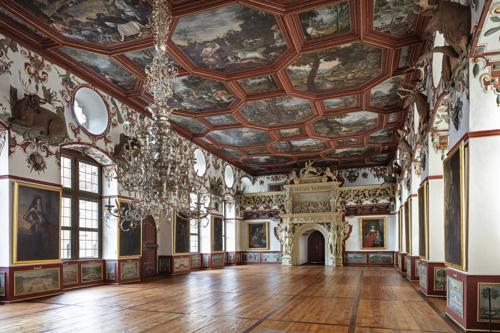
\includegraphics[height=10cm]{images/fmd10005862a.jpg}
  \caption{Knight's Hall and Room 72 - to the west}
  \label{fig:{images/fmd10005862a.jpg}}
\end{figure}

\clearpage

\begin{figure}[H]    
  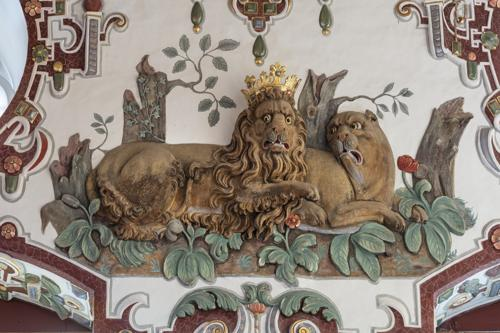
\includegraphics[height=10cm]{images/fmd10005864a.jpg}
  \caption{Lion couple – general view}
  \label{fig:{images/fmd10005864a.jpg}}
\end{figure}

\clearpage

\begin{figure}[H]    
  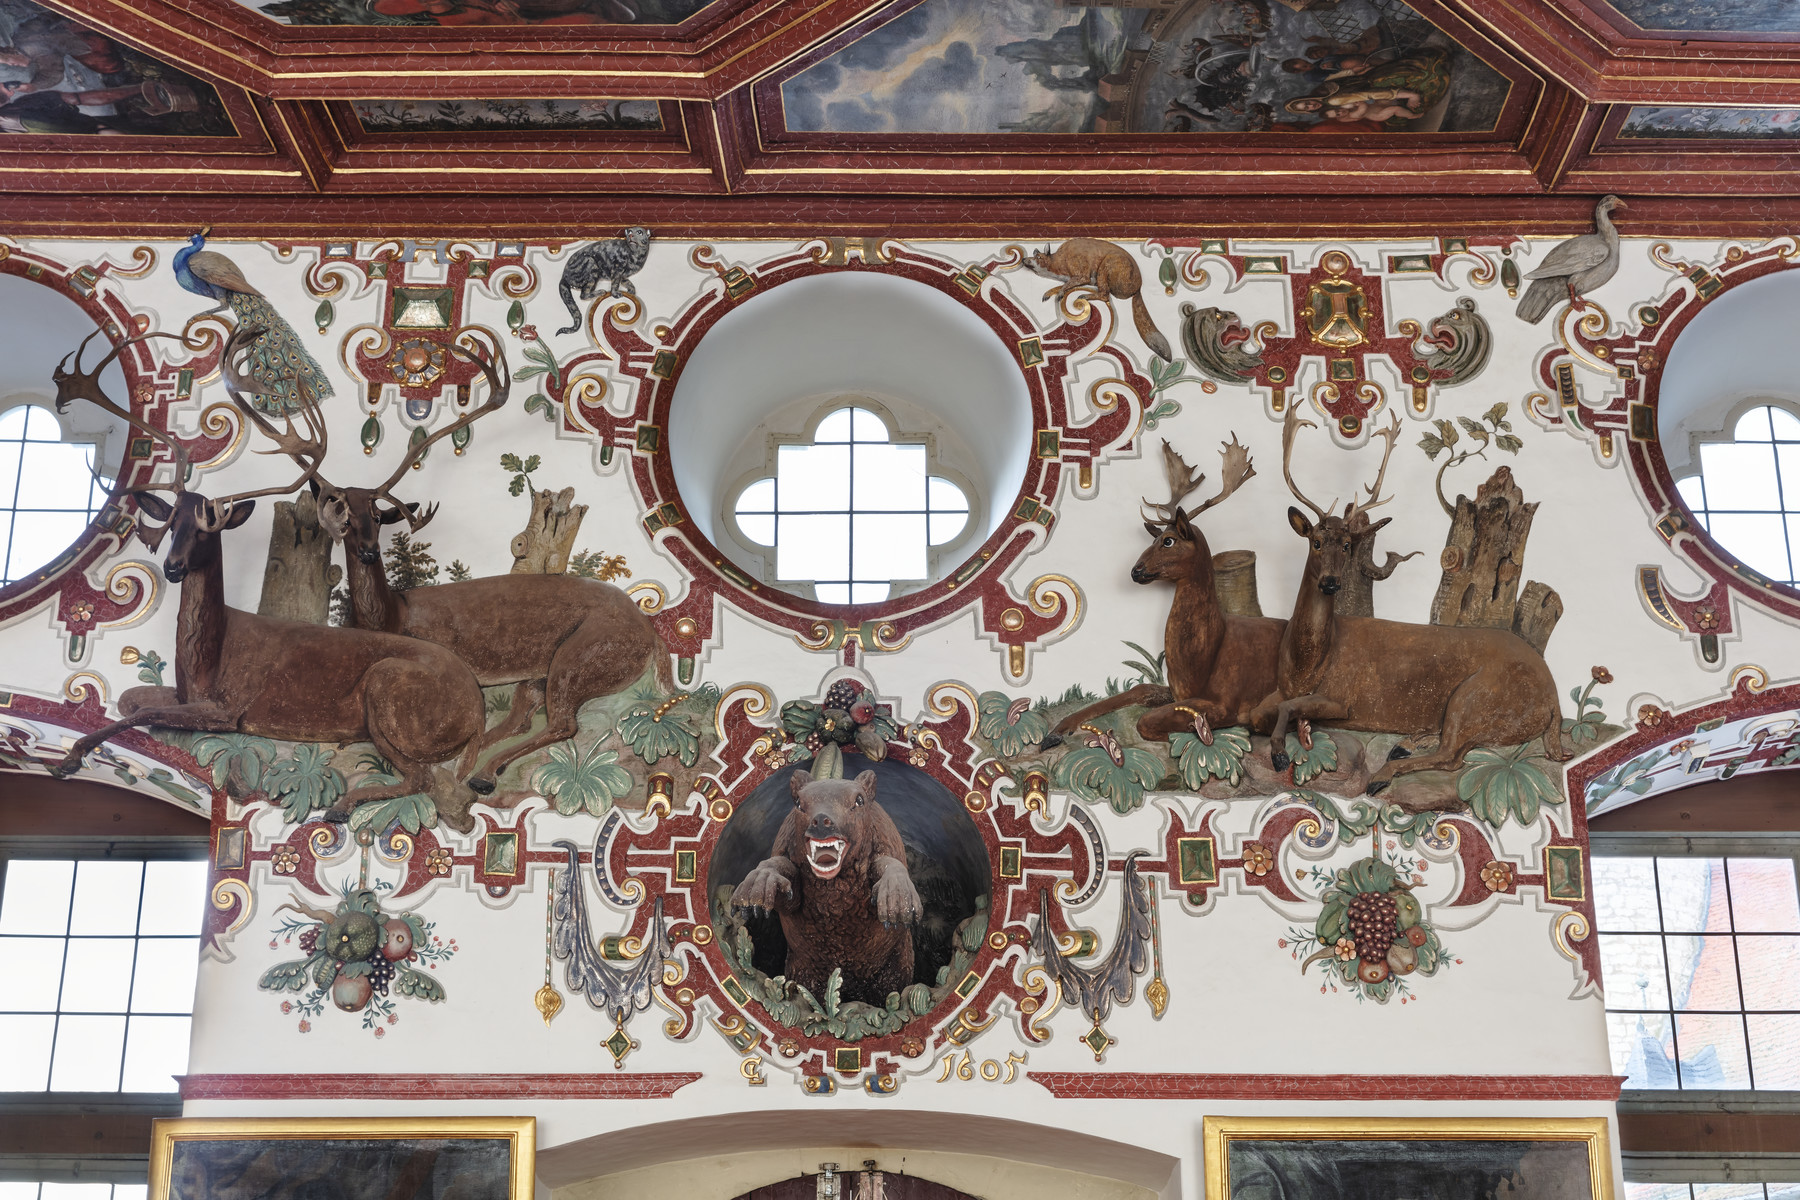
\includegraphics[height=10cm]{images/fmd10005865a.jpg}
  \caption{Bear – general view}
  \label{fig:{images/fmd10005865a.jpg}}
\end{figure}

\clearpage

\begin{figure}[H]    
  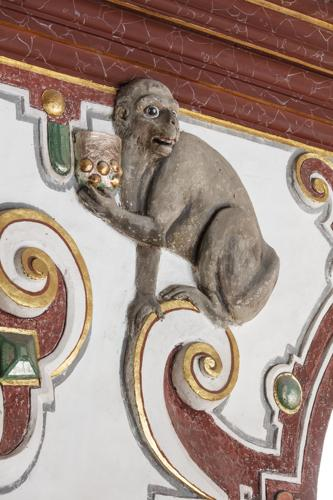
\includegraphics[height=10cm]{images/fmd10005867a.jpg}
  \caption{Monkey – general view}
  \label{fig:{images/fmd10005867a.jpg}}
\end{figure}

\clearpage

\begin{figure}[H]    
  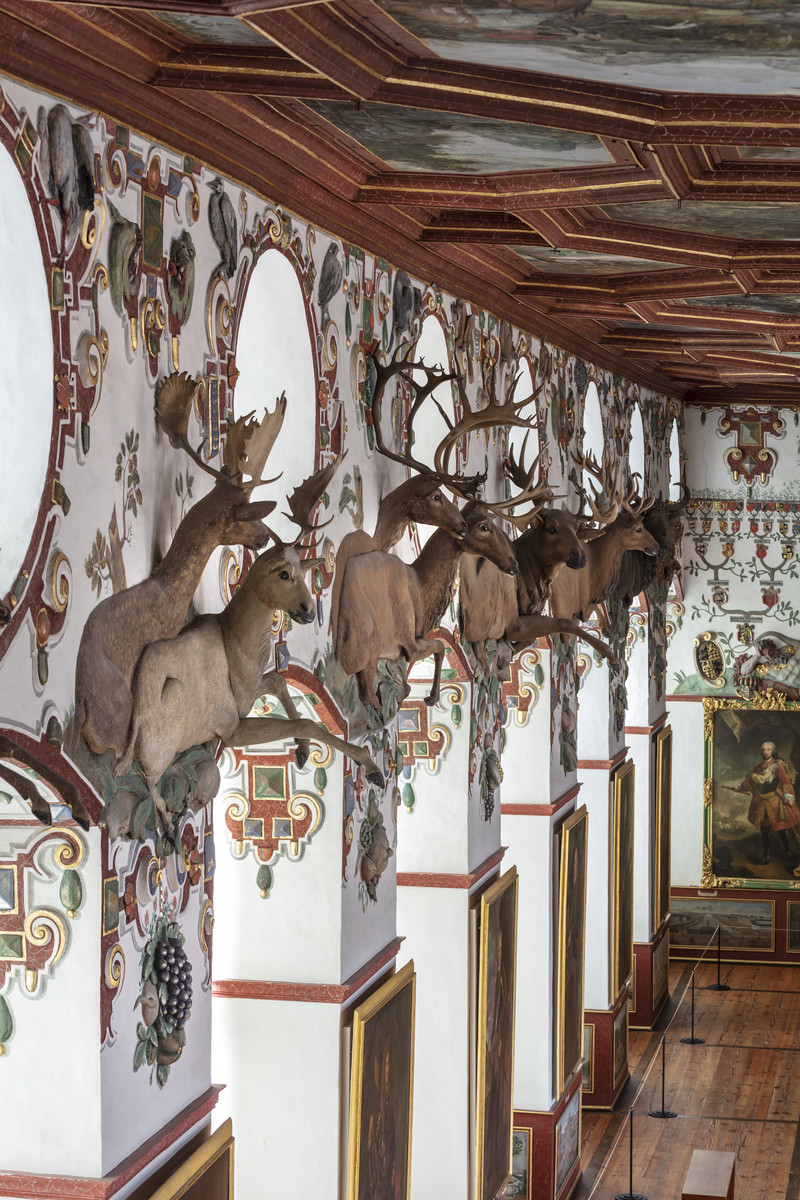
\includegraphics[height=10cm]{images/fmd10005866a.jpg}
  \caption{Deer pairs – general view}
  \label{fig:{images/fmd10005866a.jpg}}
\end{figure}

\clearpage

\begin{figure}[H]    
  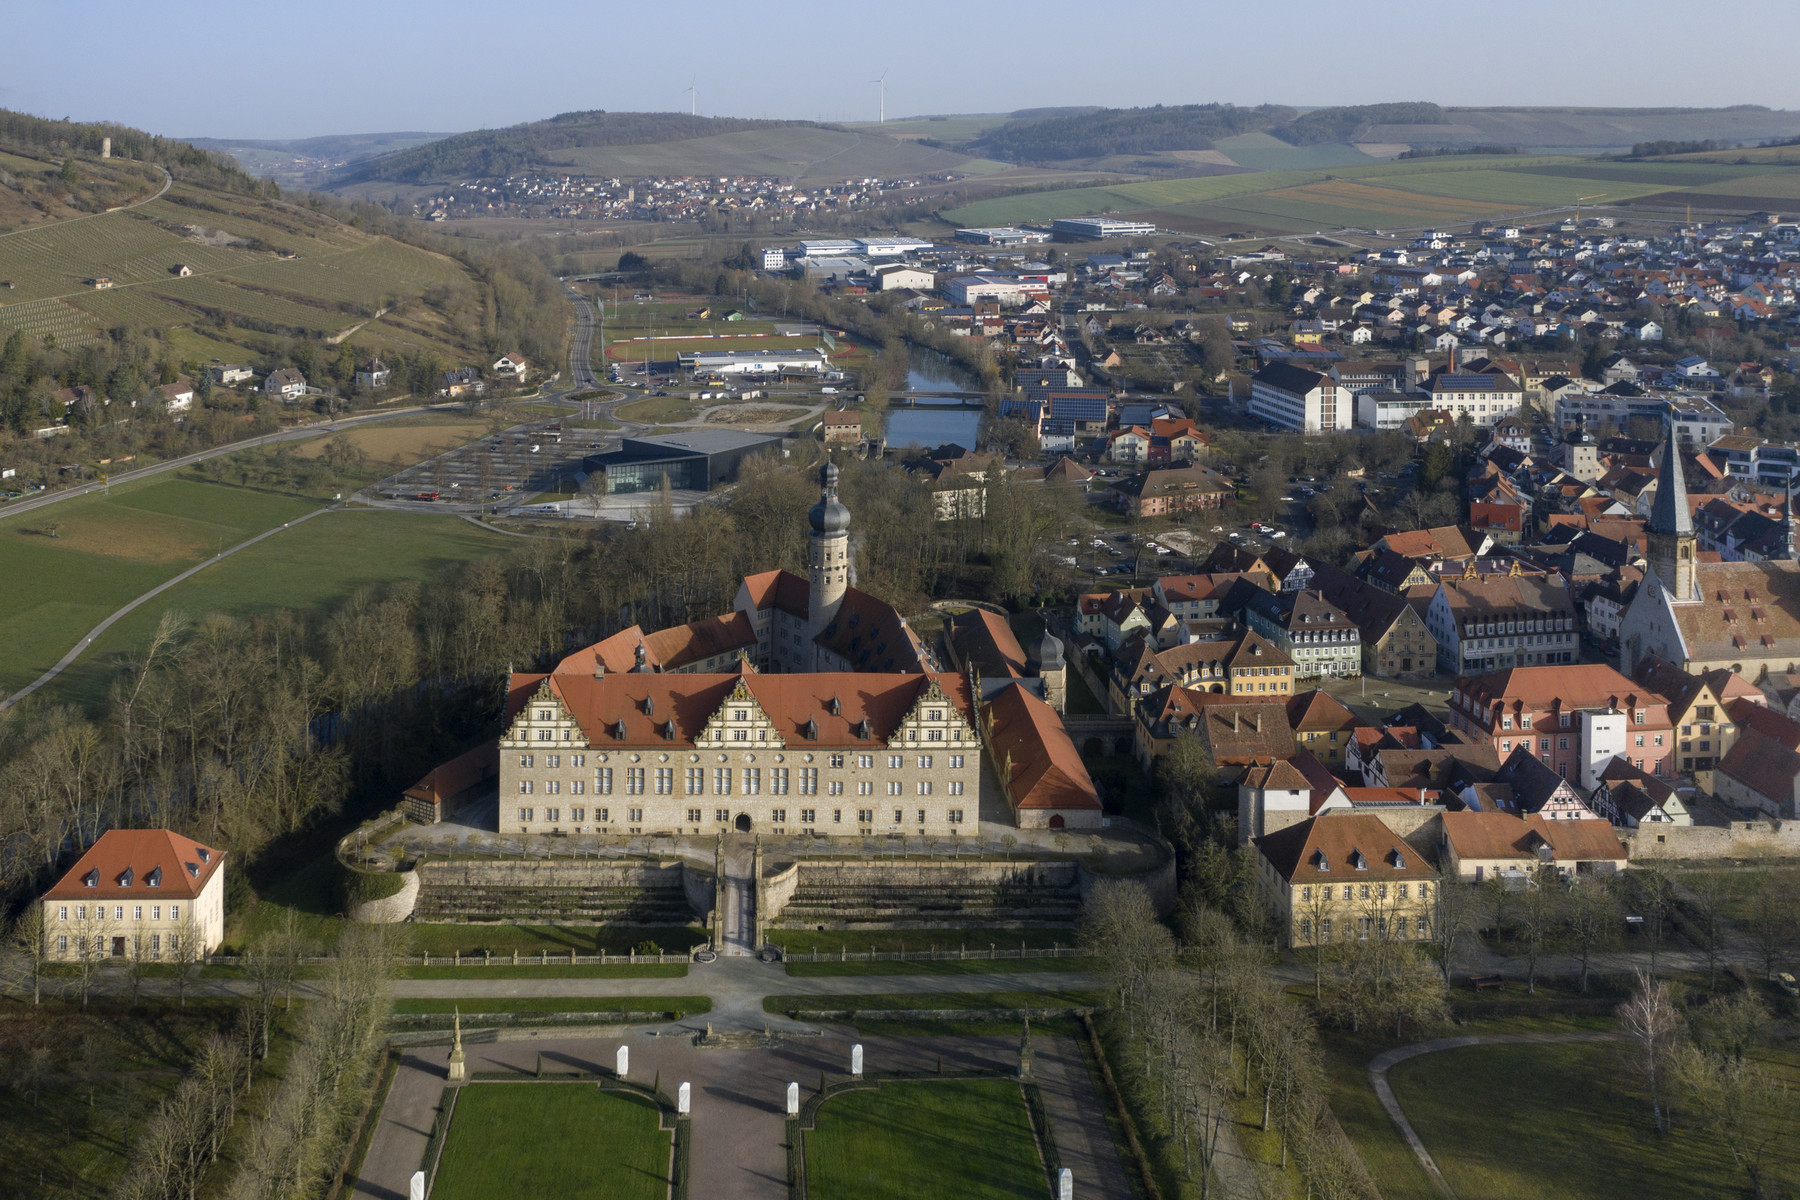
\includegraphics[height=10cm]{images/fmd10024321a.jpg}
  \caption{Hall building - garden side of the palace from the south}
  \label{fig:{images/fmd10024321a.jpg}}
\end{figure}

\clearpage

\begin{figure}[H]    
  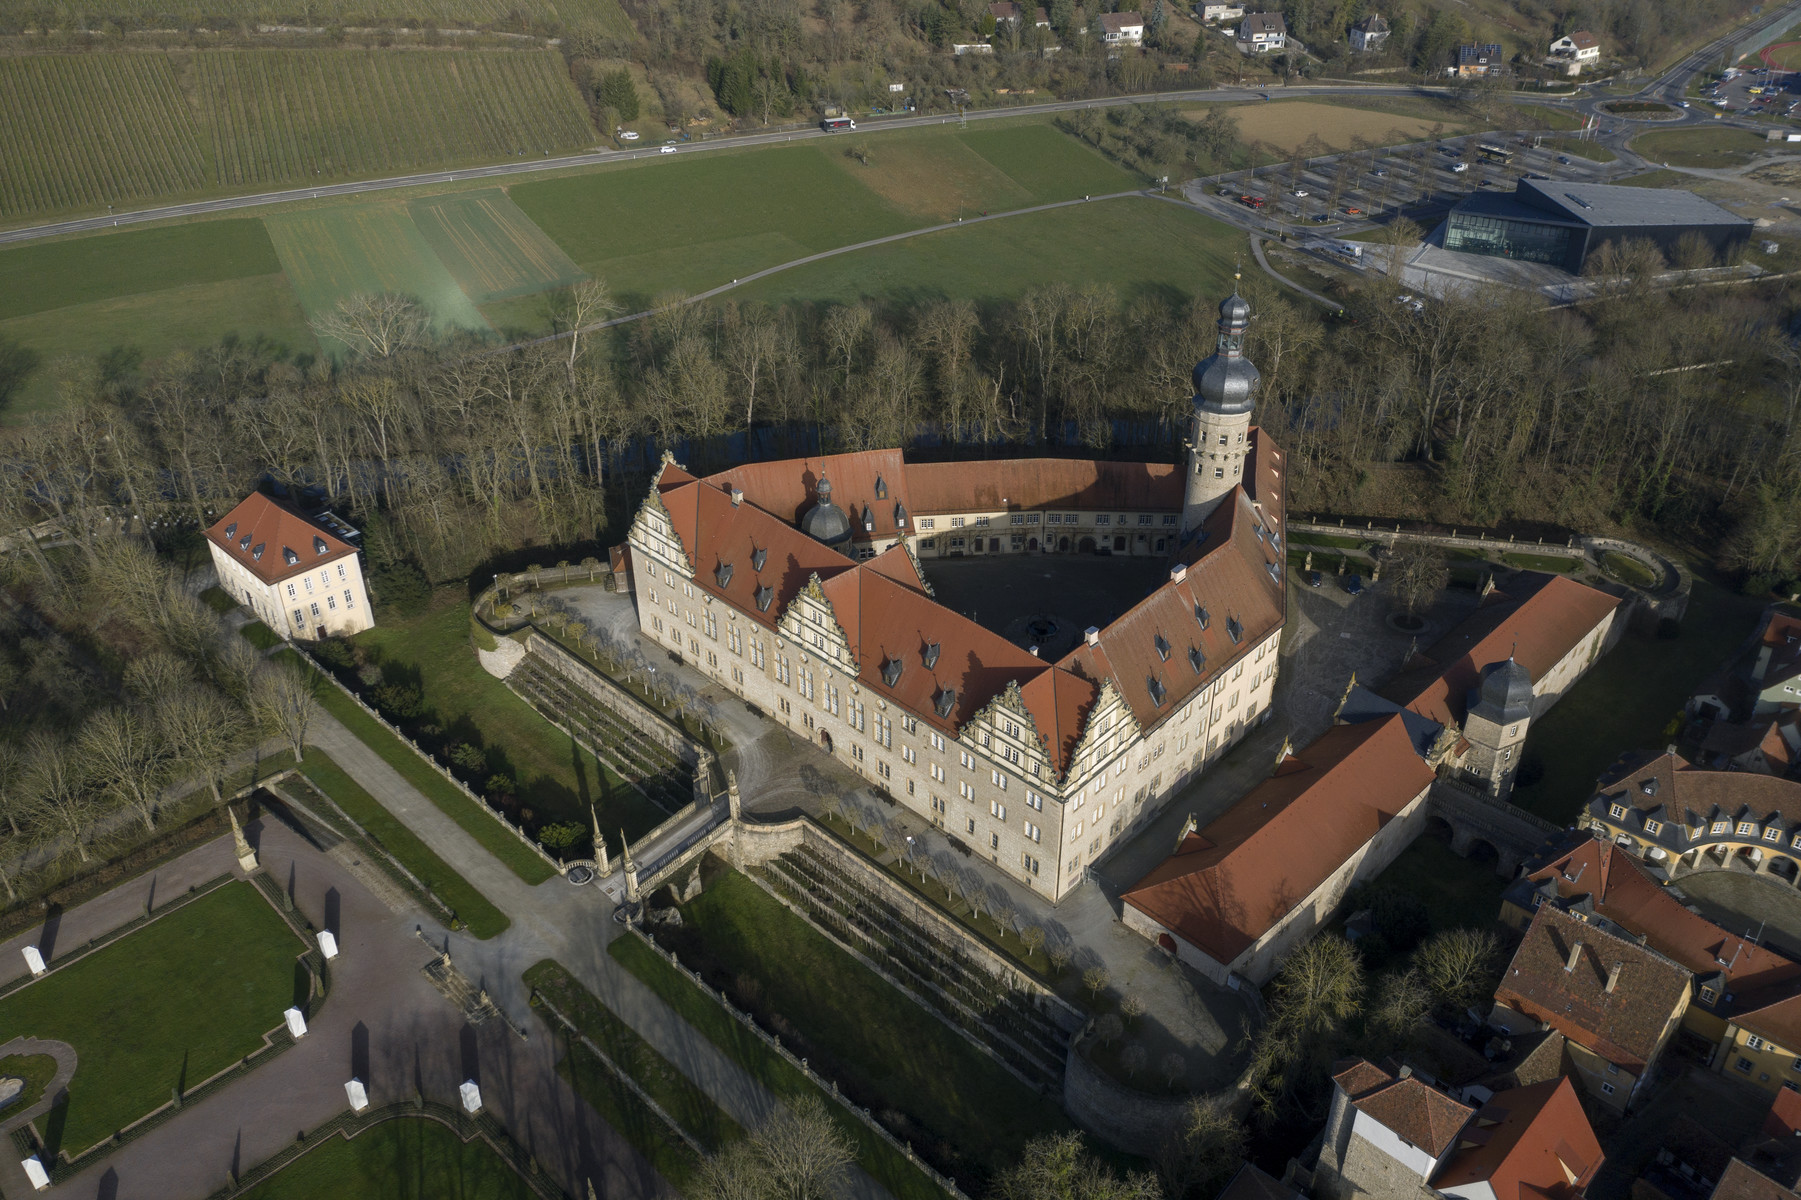
\includegraphics[height=10cm]{images/fmd10024322a.jpg}
  \caption{Saalbau - from the south-east}
  \label{fig:{images/fmd10024322a.jpg}}
\end{figure}

\clearpage

\begin{figure}[H]    
  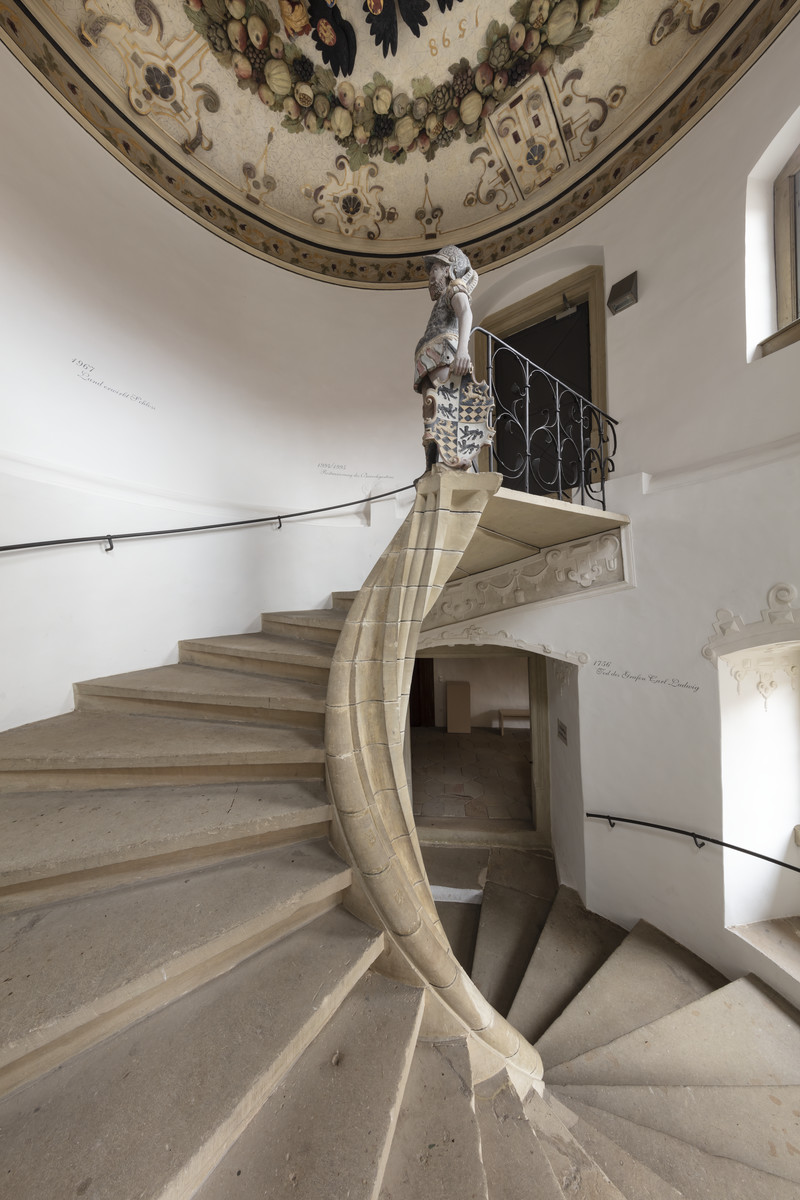
\includegraphics[height=10cm]{images/fmd10005853a.jpg}
  \caption{Development space sequences}
  \label{fig:{images/fmd10005853a.jpg}}
\end{figure}

\clearpage

\begin{figure}[H]    
  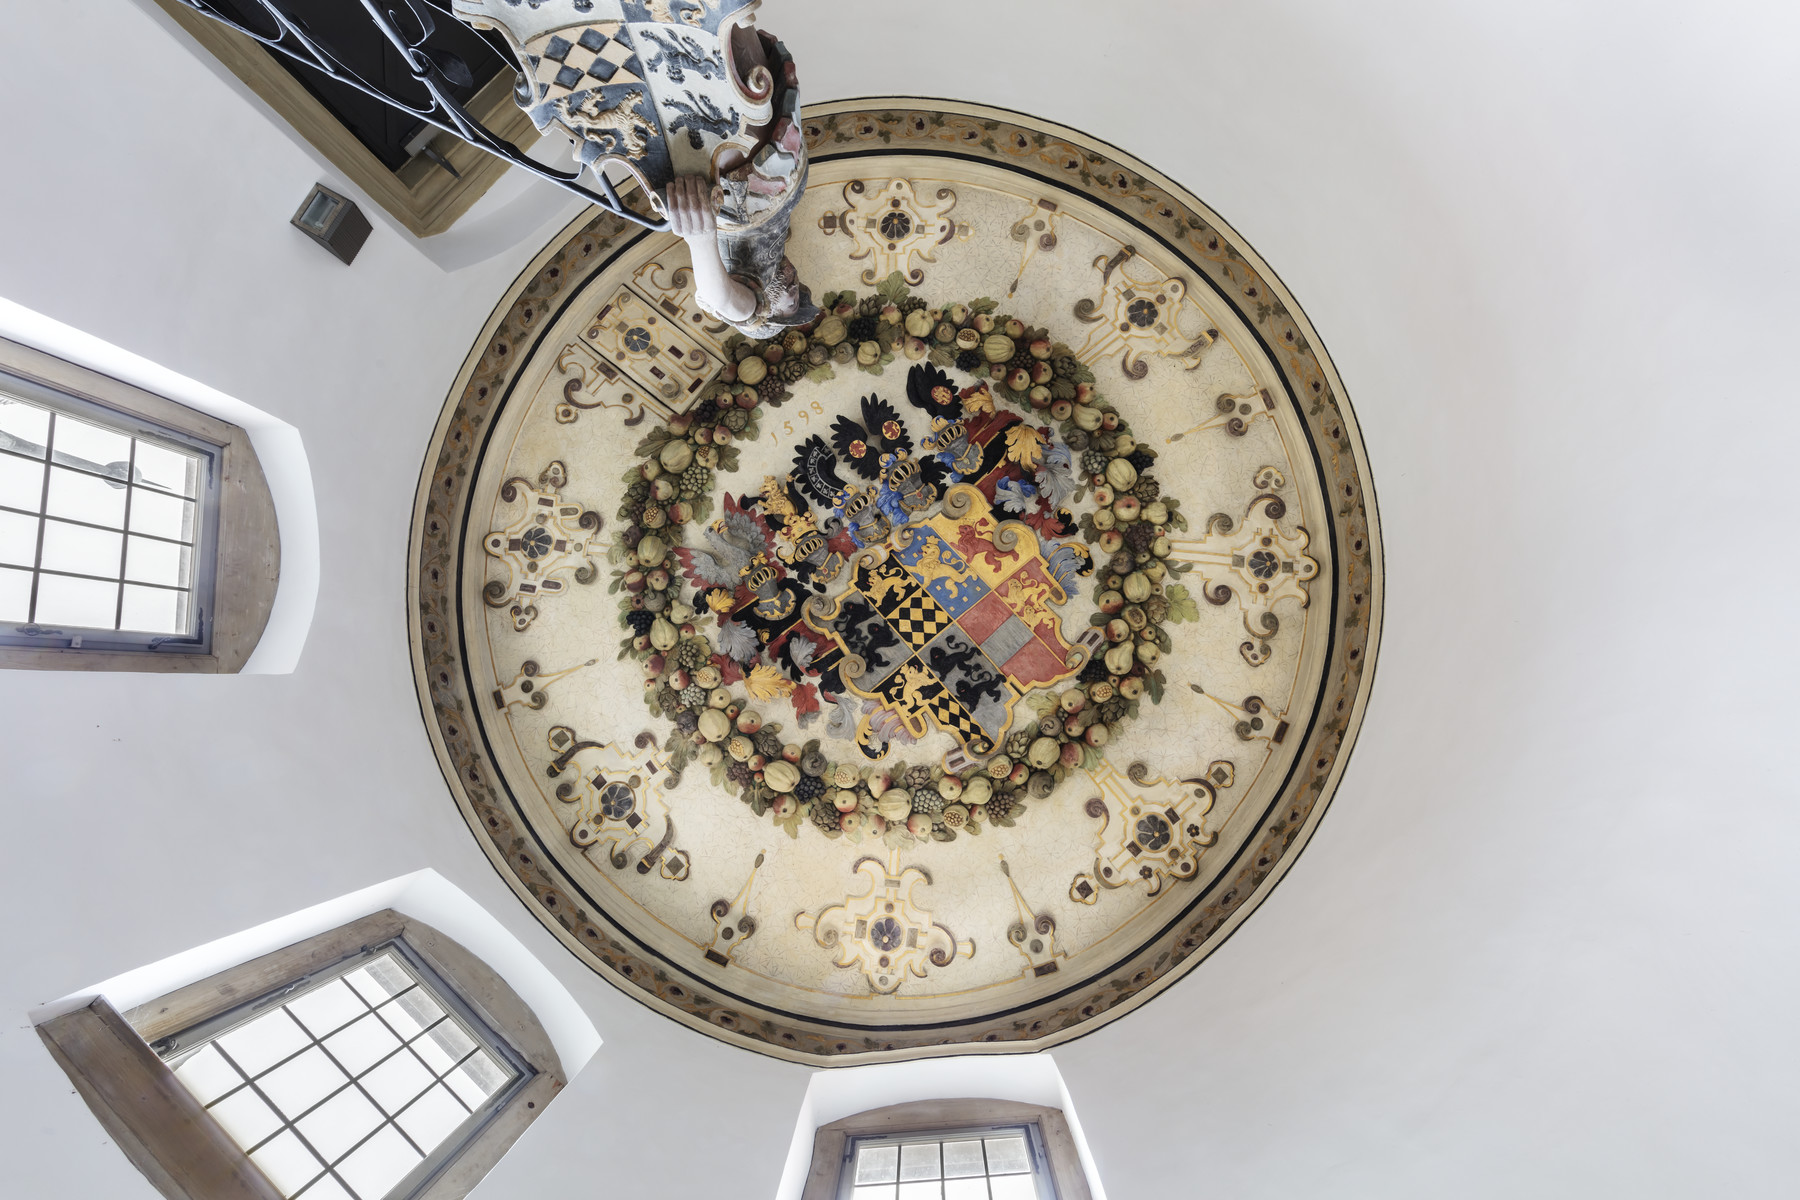
\includegraphics[height=10cm]{images/fmd10005854a.jpg}
  \caption{Ceiling decoration on stairwell}
  \label{fig:{images/fmd10005854a.jpg}}
\end{figure}

\clearpage

\begin{figure}[H]    
  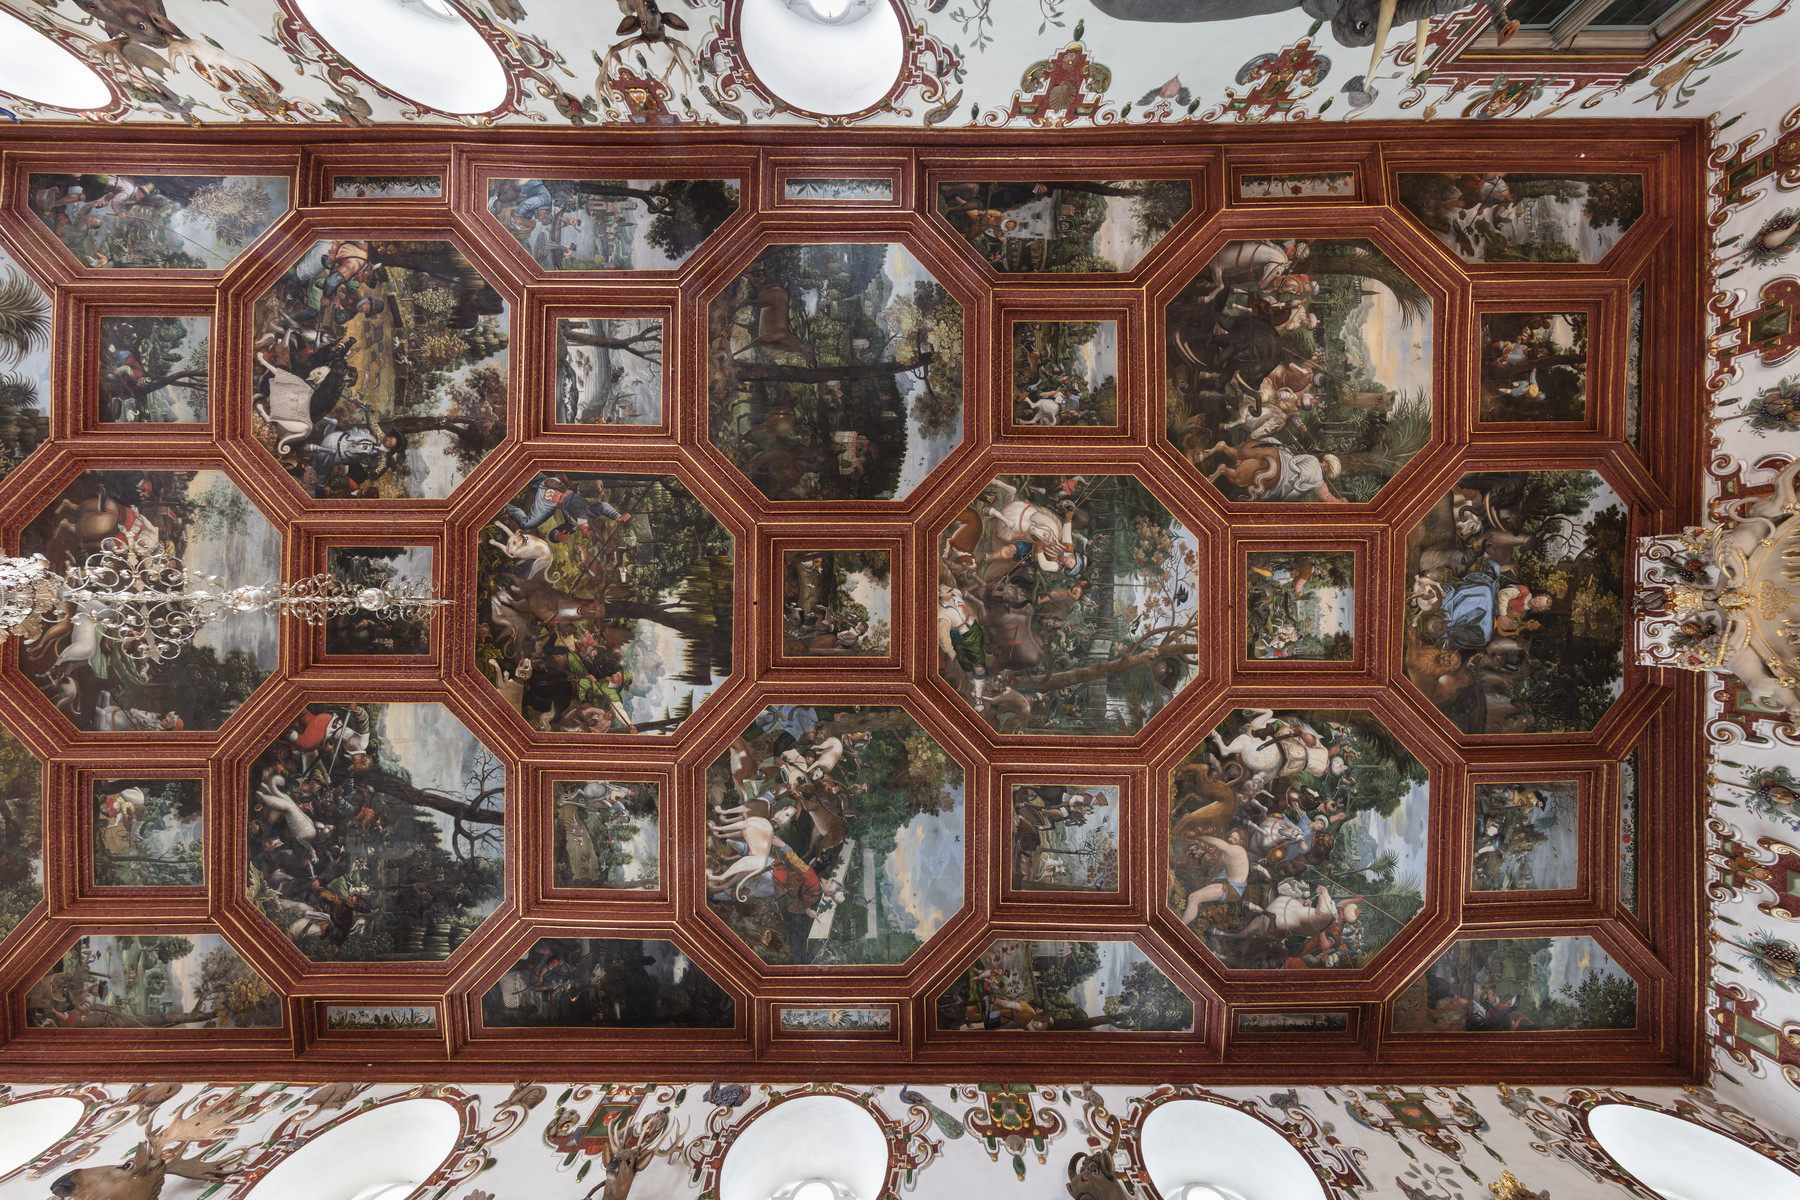
\includegraphics[height=10cm]{images/fmd10005870a.jpg}
  \caption{Ceiling Decoration of the Knights' Hall – Eastern Part of the Ceiling}
  \label{fig:{images/fmd10005870a.jpg}}
\end{figure}

\clearpage

\begin{figure}[H]    
  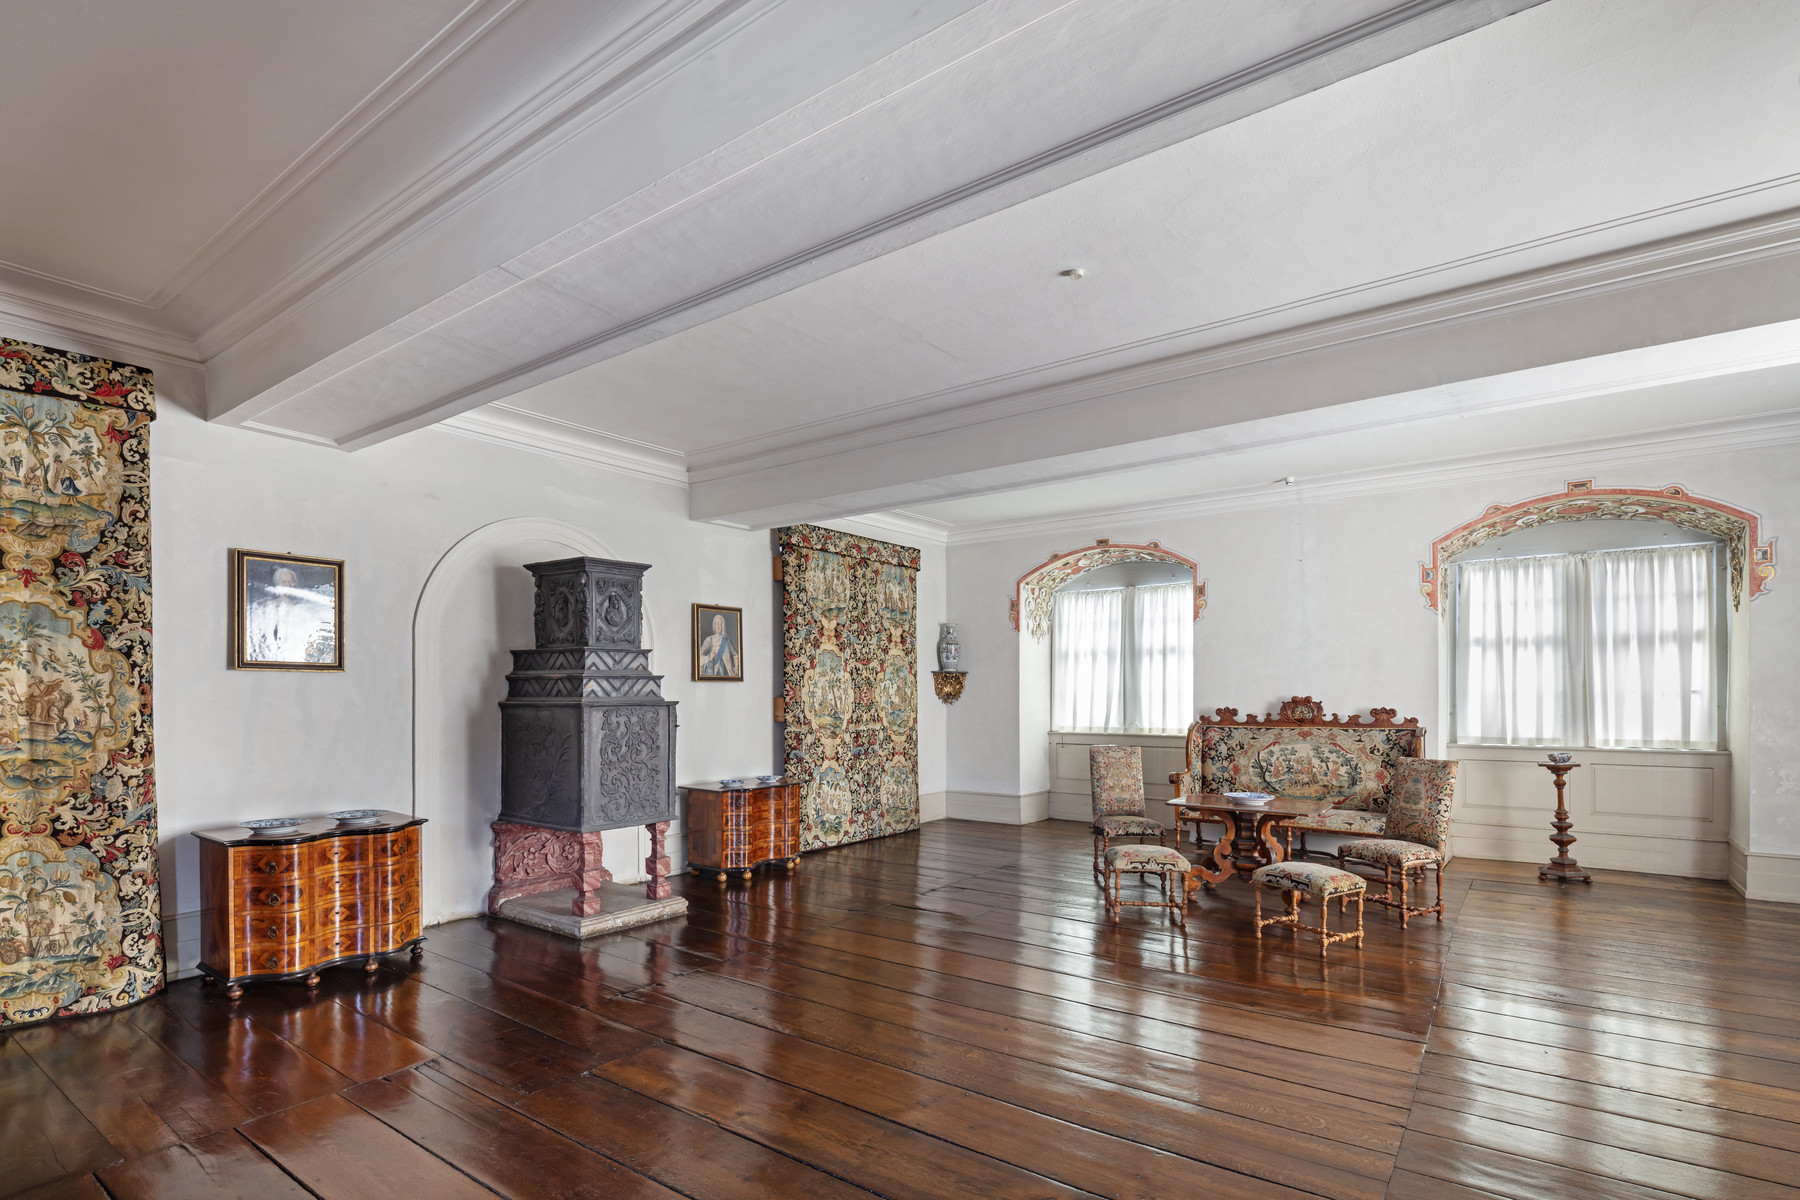
\includegraphics[height=10cm]{images/fmd10005852a.jpg}
  \caption{Einstige Tafelstube and Raum 69a – nach Südosten}
  \label{fig:{images/fmd10005852a.jpg}}
\end{figure}

\clearpage

\begin{figure}[H]    
  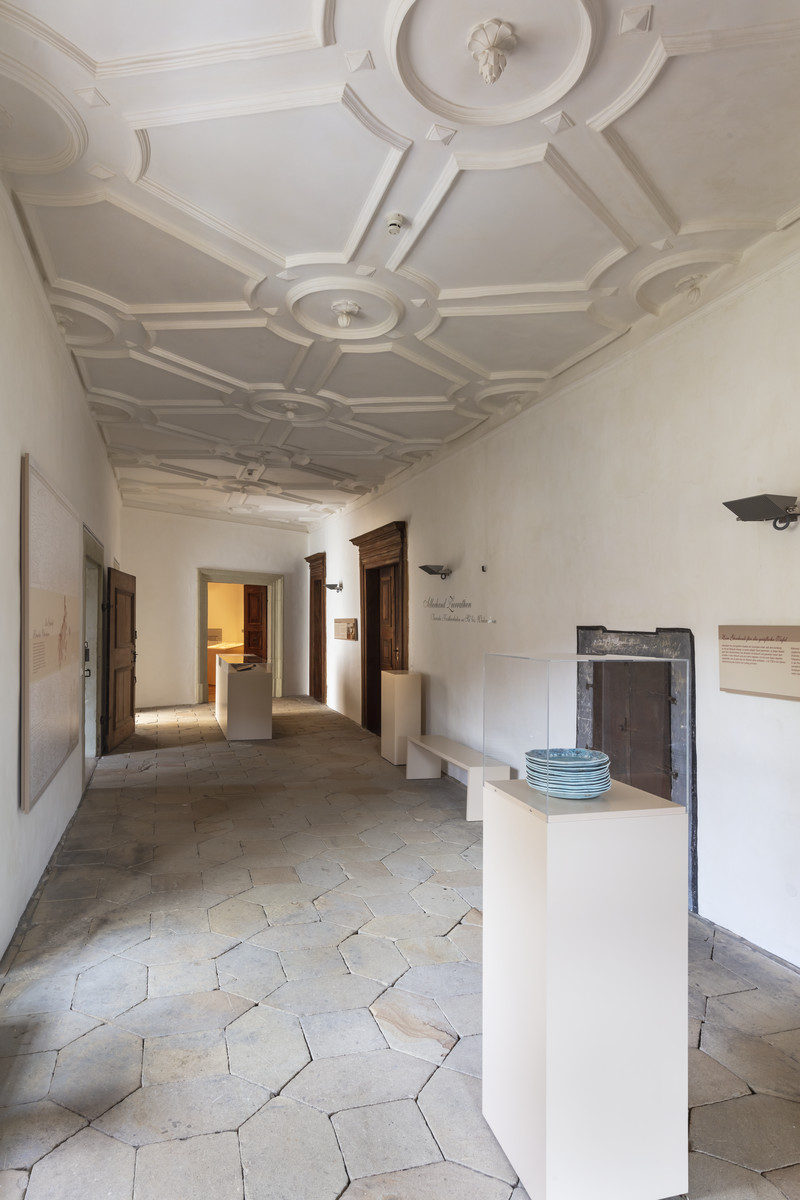
\includegraphics[height=10cm]{images/fmd10005855a.jpg}
  \caption{Der Saalbau Bild}
  \label{fig:{images/fmd10005855a.jpg}}
\end{figure}

\clearpage

\begin{figure}[H]    
  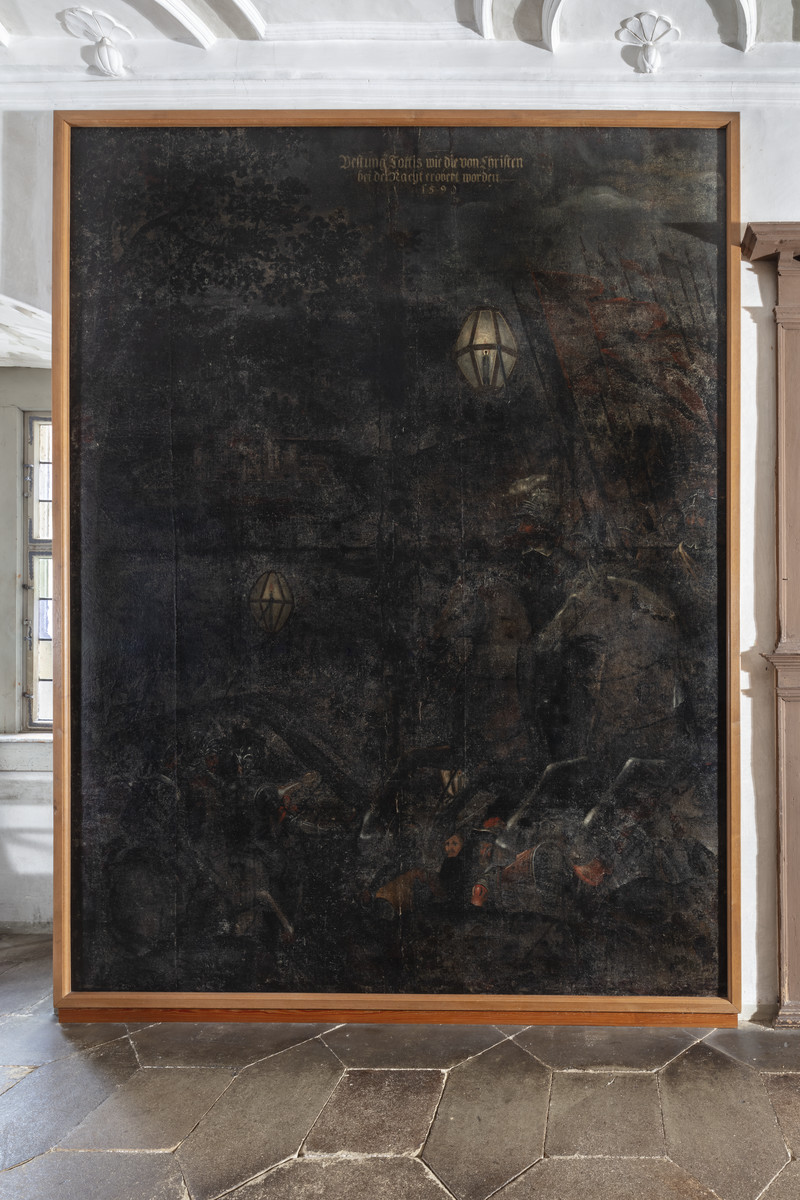
\includegraphics[height=10cm]{images/fmd10005851a.jpg}
  \caption{Eroberung der Festung Tottis – Gesamtansicht}
  \label{fig:{images/fmd10005851a.jpg}}
\end{figure}

\clearpage

\begin{figure}[H]    
  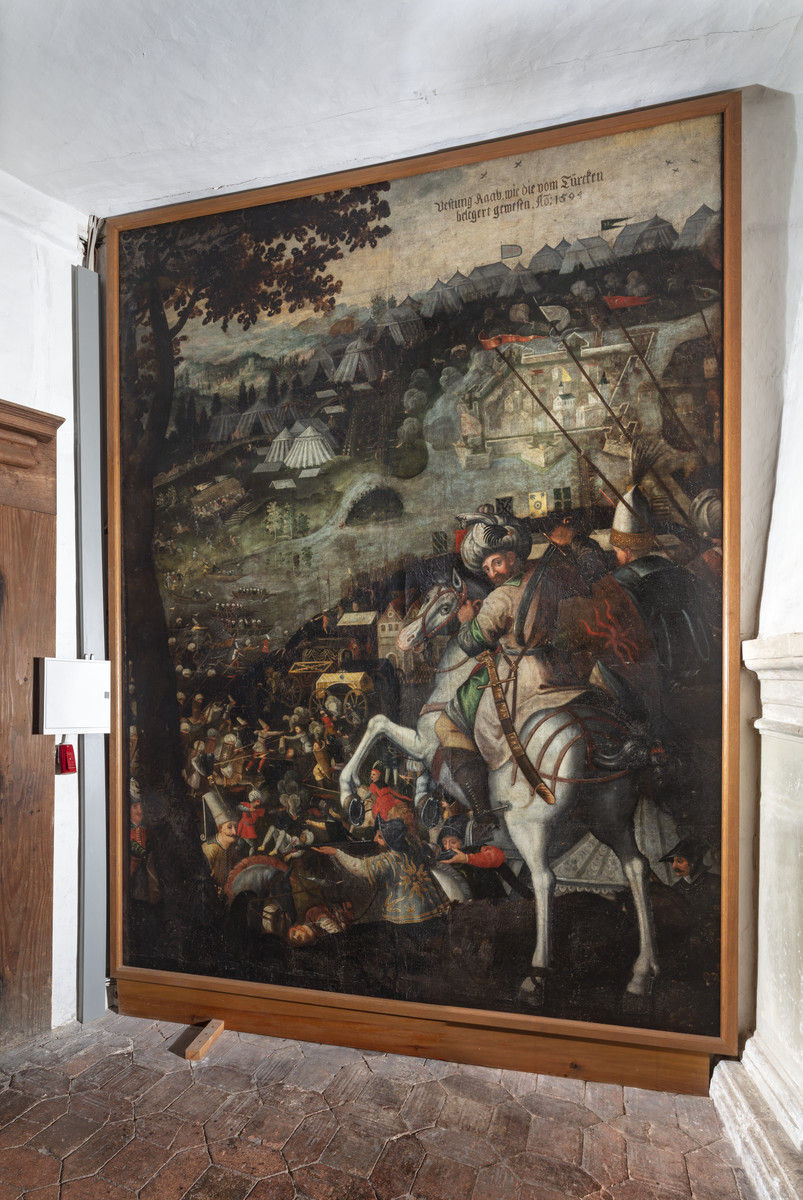
\includegraphics[height=10cm]{images/fmd10005843a.jpg}
  \caption{Belagerung der Festung Raab – Gesamtansicht}
  \label{fig:{images/fmd10005843a.jpg}}
\end{figure}

\clearpage

\begin{figure}[H]    
  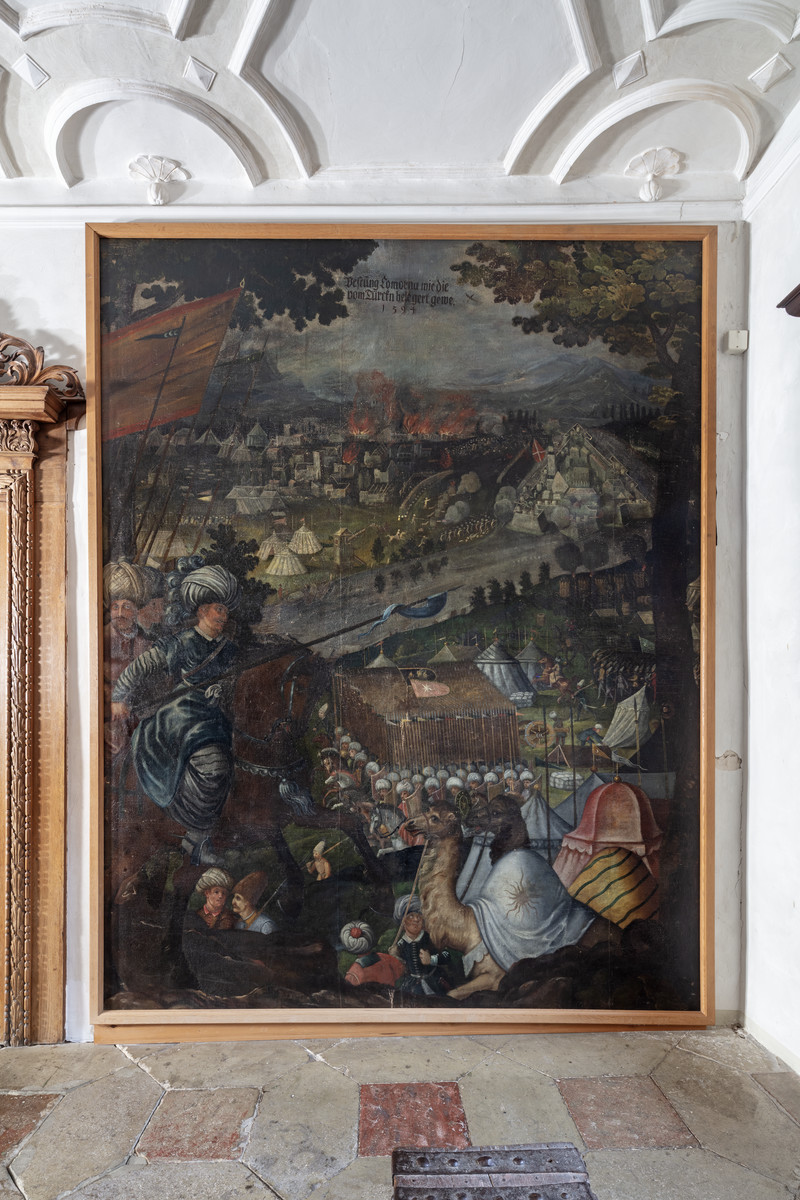
\includegraphics[height=10cm]{images/fmd10005850a.jpg}
  \caption{Belagerung der Festung Comorna – Gesamtansicht}
  \label{fig:{images/fmd10005850a.jpg}}
\end{figure}

\clearpage

\begin{figure}[H]    
  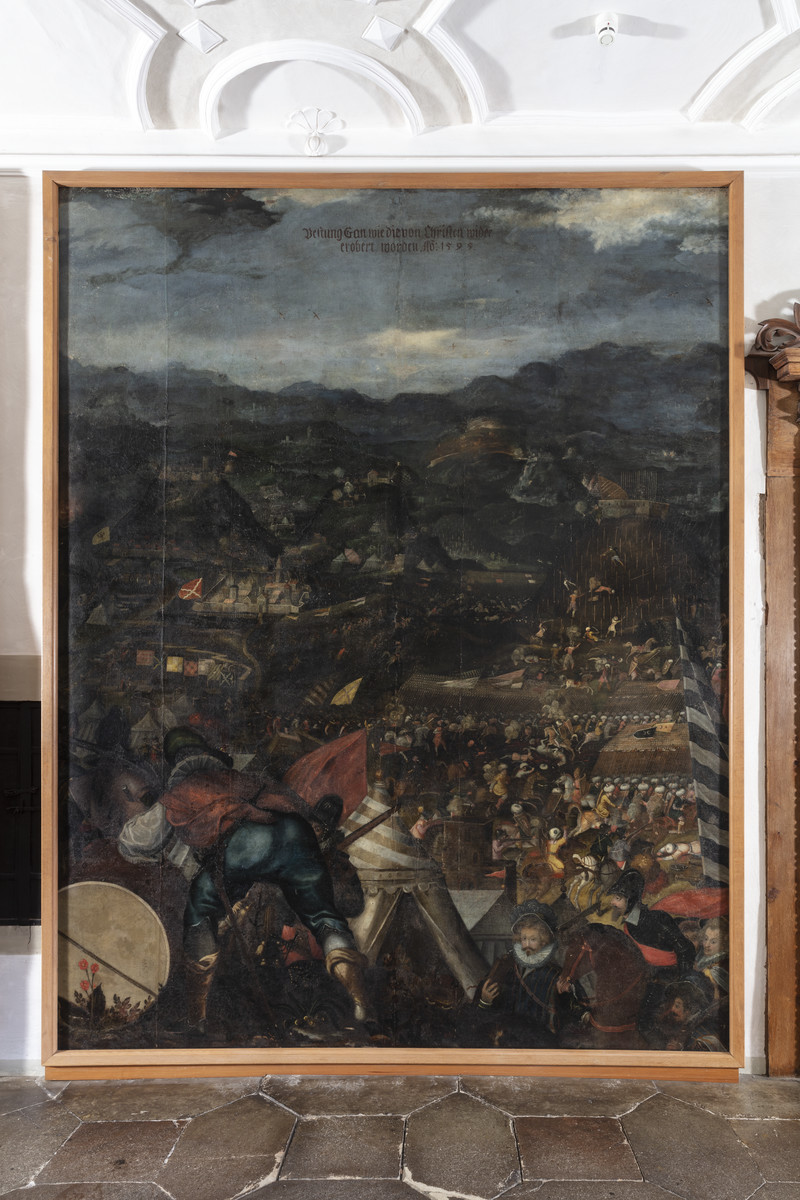
\includegraphics[height=10cm]{images/fmd10005848a.jpg}
  \caption{Eroberung der Festung Gran – Gesamtansicht}
  \label{fig:{images/fmd10005848a.jpg}}
\end{figure}

\clearpage

\begin{figure}[H]    
  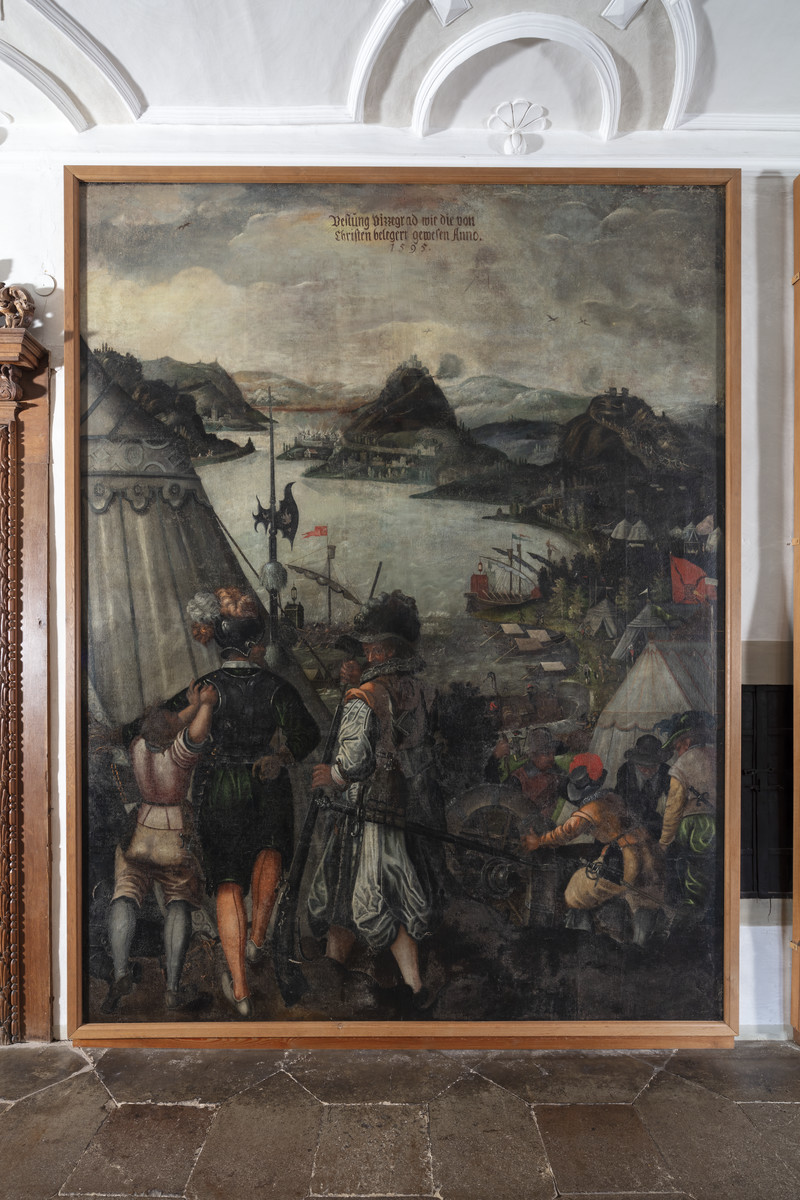
\includegraphics[height=10cm]{images/fmd10005840a.jpg}
  \caption{Belagerung der Festung von Visegrád – Gesamtansicht}
  \label{fig:{images/fmd10005840a.jpg}}
\end{figure}

\clearpage

\begin{figure}[H]    
  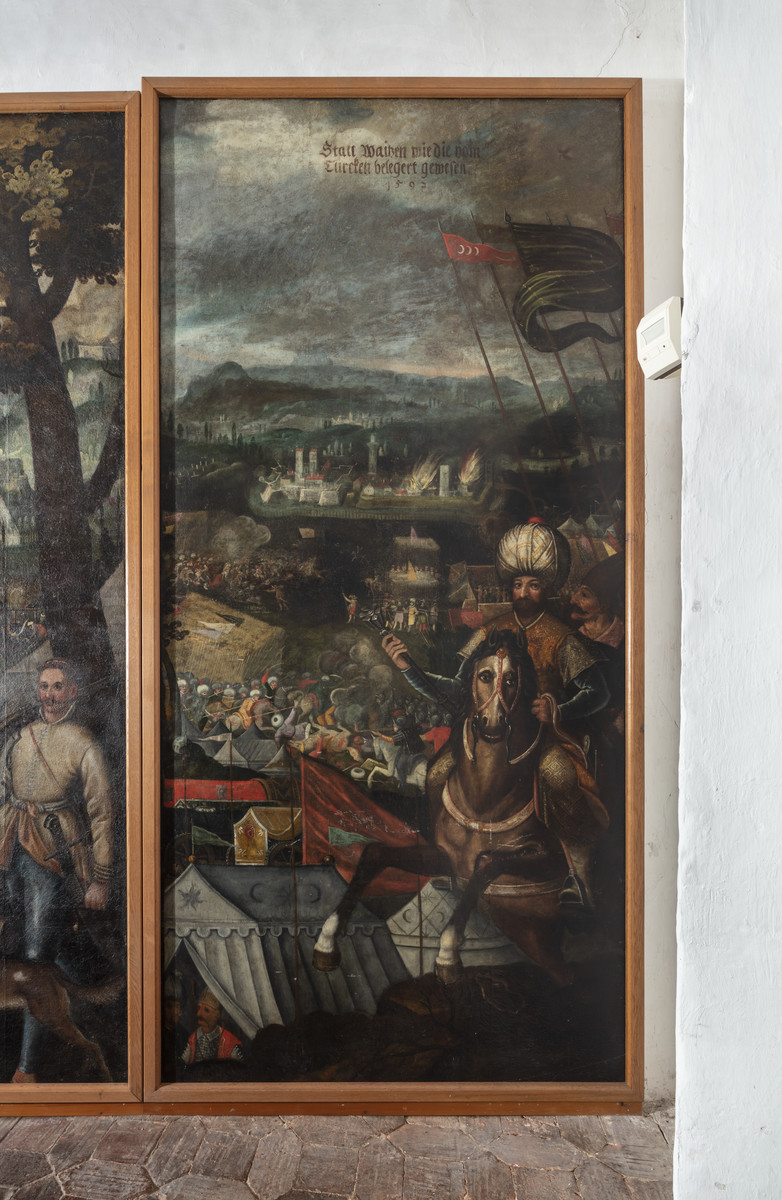
\includegraphics[height=10cm]{images/fmd10005842a.jpg}
  \caption{Belagerung der Stadt Waitzen – Gesamtansicht}
  \label{fig:{images/fmd10005842a.jpg}}
\end{figure}

\clearpage

\begin{figure}[H]    
  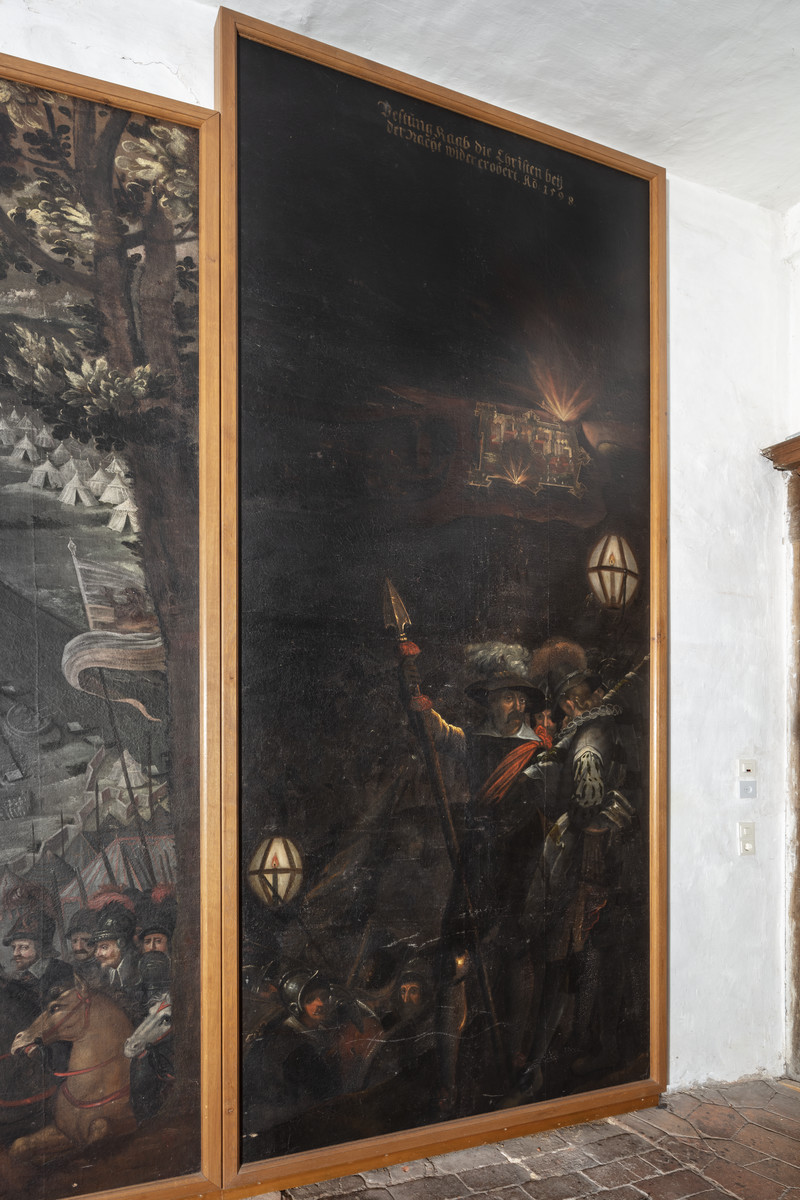
\includegraphics[height=10cm]{images/fmd10005846a.jpg}
  \caption{Wiedereroberung der Festung Raab – Gesamtansicht}
  \label{fig:{images/fmd10005846a.jpg}}
\end{figure}

\clearpage

\begin{figure}[H]    
  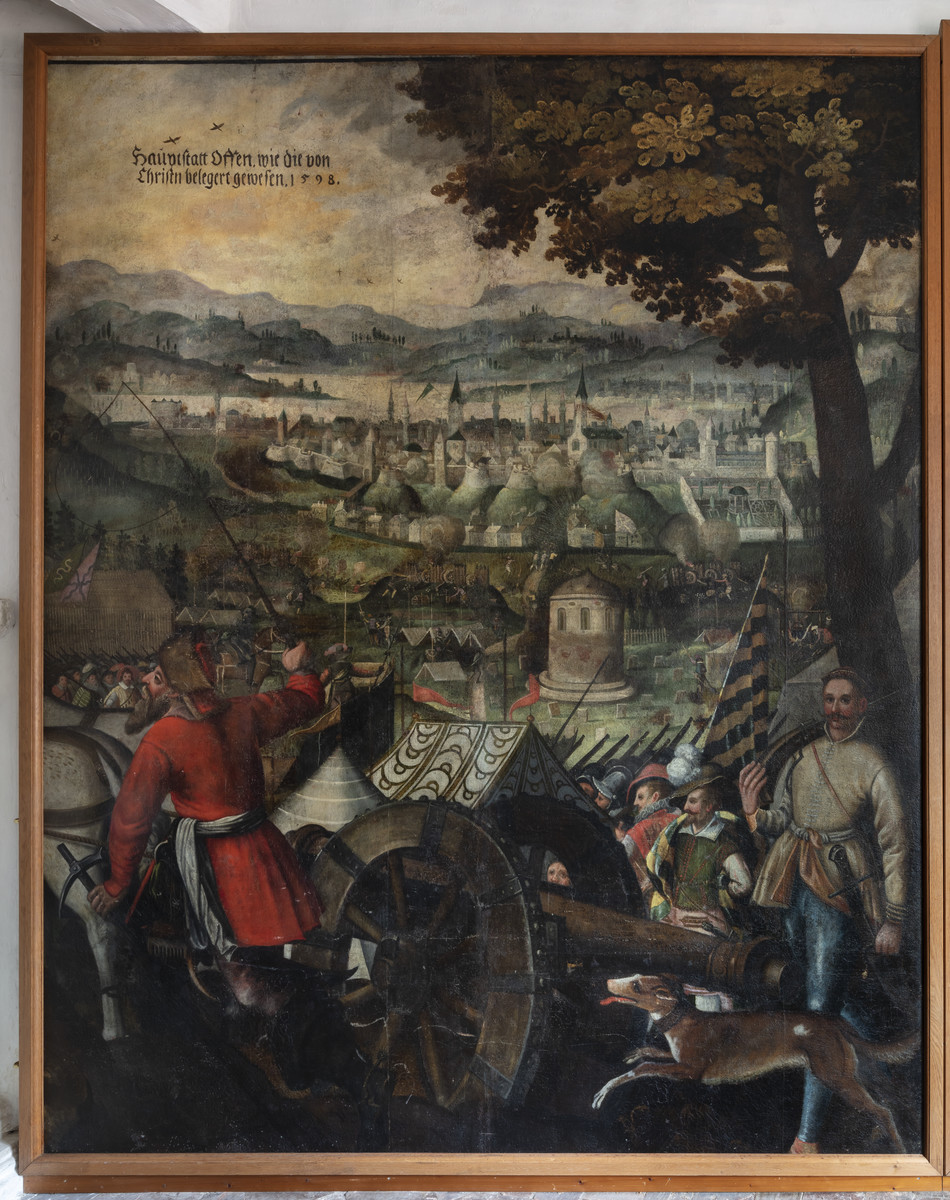
\includegraphics[height=10cm]{images/fmd10005847a.jpg}
  \caption{Belagerung der Stadt Ofen im Jahr 1598 – Gesamtansicht}
  \label{fig:{images/fmd10005847a.jpg}}
\end{figure}

\clearpage

\begin{figure}[H]    
  \includegraphics[height=10cm]{images/fmd10005844a.jpg}
  \caption{Belagerung der Stadt Ofen im Jahr 1603 – Gesamtansicht}
  \label{fig:{images/fmd10005844a.jpg}}
\end{figure}

\clearpage

\begin{figure}[H]    
  \includegraphics[height=10cm]{images/fmd10005845a.jpg}
  \caption{Belagerung der Festung Gran – Gesamtansicht (Anno 1604)}
  \label{fig:{images/fmd10005845a.jpg}}
\end{figure}

\clearpage

\begin{figure}[H]    
  \includegraphics[height=10cm]{images/fmd10005849a.jpg}
  \caption{Scharmützel bei der Belagerung der Stadt Ofen im Jahr 1603 – Gesamtansicht}
  \label{fig:{images/fmd10005849a.jpg}}
\end{figure}

\clearpage

\begin{figure}[H]    
  \includegraphics[height=10cm]{images/fmd10005841a.jpg}
  \caption{Belagerung der Festung Gran – Gesamtansicht (1594)}
  \label{fig:{images/fmd10005841a.jpg}}
\end{figure}

\clearpage

\begin{figure}[H]    
  \includegraphics[height=10cm]{images/fmd10005861a.jpg}
  \caption{Die barocken Schloss- und Gartenveduten bild}
  \label{fig:{images/fmd10005861a.jpg}}
\end{figure}

\clearpage

\begin{figure}[H]    
  \includegraphics[height=10cm]{images/fmd10005863a.jpg}
  \caption{Die barocken Schloss- und Gartenveduten bild 2}
  \label{fig:{images/fmd10005863a.jpg}}
\end{figure}

\clearpage

\begin{figure}[H]    
  \includegraphics[height=10cm]{images/fmd10024323a.jpg}
  \caption{Orpheus with the lyre and the animals under a tree}
  \label{fig:{images/fmd10024323a.jpg}}
\end{figure}

\clearpage

\begin{figure}[H]    
  \includegraphics[height=10cm]{images/fmd10024324a.jpg}
  \caption{Otter catching, with Weikersheim Castle in the background – on the left, duck hunting, on the right, otter catching}
  \label{fig:{images/fmd10024324a.jpg}}
\end{figure}

\clearpage

\begin{figure}[H]    
  \includegraphics[height=10cm]{images/fmd10024322a.jpg}
  \caption{Schloss}
  \label{fig:{images/fmd10024322a.jpg}}
\end{figure}

\clearpage

\begin{figure}[H]    
  \includegraphics[height=10cm]{images/fmd10005902a.jpg}
  \caption{Schloss Weikersheim}
  \label{fig:{images/fmd10005902a.jpg}}
\end{figure}

\clearpage

\begin{figure}[H]    
  \includegraphics[height=10cm]{images/fmd10024325a.jpg}
  \caption{Wildkatzenjagd - General view}
  \label{fig:{images/fmd10024325a.jpg}}
\end{figure}

\clearpage

\begin{figure}[H]    
  \includegraphics[height=10cm]{images/fmd10024325a.jpg}
  \caption{Orpheus with the Lyre and the Animals under a Tree - General View}
  \label{fig:{images/fmd10024325a.jpg}}
\end{figure}

\clearpage

\begin{figure}[H]    
  \includegraphics[height=10cm]{images/fmd10005859a.jpg}
  \caption{Knight's Hall and Room 72 - to the east}
  \label{fig:{images/fmd10005859a.jpg}}
\end{figure}

\clearpage

\begin{figure}[H]    
  \includegraphics[height=10cm]{images/fmd10005860a.jpg}
  \caption{Knight's Hall and Room 72 - to the east}
  \label{fig:{images/fmd10005860a.jpg}}
\end{figure}

\clearpage

\end{figure*}%


\backmatter


\end{document}
